\chapter{Perspective \& Future Directions}

In chapters \ref{chapter:processor_characterization} and \ref{chapter:grover_algorithm} we demonstrated a universal two-qubit gate on our quantum processor and used it to realize the two-qubit Grover search algorithm, achieving probabilistic quantum speed-up. However, this approach to quantum computing cannot be scaled beyond a few qubits, wich is mostly due to the nature of the qubit-qubit coupling that has been chosen: The direct capacitive coupling produces a qubit-qubit interaction which is always on and whose amplitude decreases as $g_{qq}/\Delta_{qq}$. To be able to realize gate times which are shorter than the typical coherence time of Transmon qubits (typically $T_1,T_\phi \simeq\ 1-10 \;\mathrm{\mu s}$) we require coupling strengts $g_{qq}/2\pi \ge 10\;\mathrm{MHz}$. Therefore, in order to switch of spurious coupling between any two qubits below the 5 \% level, a detuning of $\Delta_{qq}\ge 20g \simeq 200\;\mathrm{MHz}$. For a processor where one would couple a large number of qubits using this scheme, the required qubit-qubit detunings would quickly lead to so-called {\it frequency crowding}, i.e. a shortage of available working point frequencies for the different qubits of the processor.

\smallskip

Hence, for a larger-scale quantum processor, it is essential to devise a coupling scheme which allows to deterministically turn on and off the coupling between arbitary qubits. In the literature, several architectures have been proposed for this, using e.g. a parametric coupling between qubits \citep{bertet_parametric_2006} or relying on the storage of quantum information stored in the qubits in a seperate entity, such as a superconducting resonator \citep{galiautdinov_resonatorzero-qubit_2012,mariantoni_implementing_2011}.

\smallskip

In the following section, we will propose a different approach to scalable quantum computing, based on a recently introduced double Transmon qubit \citep{gambetta_superconducting_2011,srinivasan_tunable_2011} and using a fixed-frequency, microwave-tunable qubit-qubit coupling scheme as well as a single-shot readout method for individual qubits.

\smallskip

After shortly discussing our proposed architecture, we discuss recent developments in superconducting quantum computing and put them in context with our work, indicating possible future research directions.

\section{Designing a Scalable Architecture for Quantum Bits} \label{section:scalable_architecture}

In this section we describe our proposal for a scalable multi-qubit architecture based on superconducting Transmon qubits and fulfilling all of DiVincenzo's criteria for the realization of a quantum computer, as discussed in section \ref{section:divincenzo_criteria}. \citep{steane_how_2007}

\subsection{Requirements \& Problem Statement}

A scalable architecture for quantum computing should fulfill all criteria discussed above and, in addition do not incur an exponential experimental overhead for each qubit that is added to the quantum computer \citep{blume-kohout_climbing_2002}. Today, the two issues that are not addressed well by current qubit architectures, such as the quantum bus architecture used by many groups today \citep{dicarlo_demonstration_2009,wallraff_strong_2004}, which concern the qubit-qubit coupling and the readout of individual qubits. The quantum bus architecture, for instance, has an always-on coupling scheme between the qubits described by eq. (\ref{eq:cqed_bus_coupling}) which makes it hard to precisely control the coupling between individual qubits if a large number of them is present. Also, the readout of the qubit register is usually performed as a joint readout of the whole qubit register, thereby not allowing the read out of individual qubits. To summarize, a scalable superconducting qubit architecture needs to have the following properties:

\begin{enumerate}
\item Well-defined qubits with long coherence times.
\item A single-shot, high-fidelity readout method for individual qubits.
\item High-fidelity single-qubit frequency and drive control.
\item Tunable and robust qubit-qubit coupling between any two qubits.
\item Sub-exponential scaling of resources when adding more qubits to the computer.
\end{enumerate}

The current CQED architectures usually fulfill (to varying degress) properties 1, 2, 3 \& 4 but usually are not easily scalable to beyond a certain number of qubits. In this work, we have shown how the CQED architecture can be complemented with a single-shot individual qubit readout and have demonstrated the implementation of a simple quantum algorithm making use of such a readout scheme. However, the presented quantum processor is not scalable because it does not fulfill property 4: Since The qubit-qubit coupling decreases as a function of the detuning $\Delta$ as $1/\Delta$, it becomes increasingly difficult and eventually impossible to deterministically switch on and off the coupling between individual qubits when increasing their number, due to the limited available frequency space that can be allocated to each qubit (so-called {\it frequency crowding}). Also, keeping track of all involved qubit phases and frequencies incurs an overhead which increases exponentially with their number \citep{galiautdinov_resonatorzero-qubit_2012}. Using a resonator as a quantum bus to couple individual qubits does not remedy this problem.

\smallskip

In the following sections, we therefore discuss a proposal for complementing the current CQED architectures with the missing elements, putting special emphasis on a tunable qubit-qubit coupling scheme and the implementation of single-shot readout for individual qubits.

\section{Architecture Proposal}

Our proposed architecture follows the general CQED principles in that it uses Transmon qubits which are coupled to each other via a resonator that acts as a quantum bus. However, instead of using a single Transmon to represent each logical qubit, we use two of them which are capacitively coupled to each other and act as a qubit ``molecule''. As shown by Gambetta {\it et. al.}, if we couple the two Transmons of such a molecule to the quantum bus with the same coupling constant, we can use symmetry properties of the eigenstates of the double Transmon to fully cancel the coupling of the logical qubit to the bus \citep{gambetta_superconducting_2011}. This allows us to remedy the problem of frequency crowding since multiple qubits can occupy the same frequency band while remaining decoupled. In the following section we discuss in detail the properties of our logical qubit and the proposed coupling scheme.

\subsection{The Double Transmon} \label{section:double_transmon}

\begin{figure}[ht!]
	\centering
	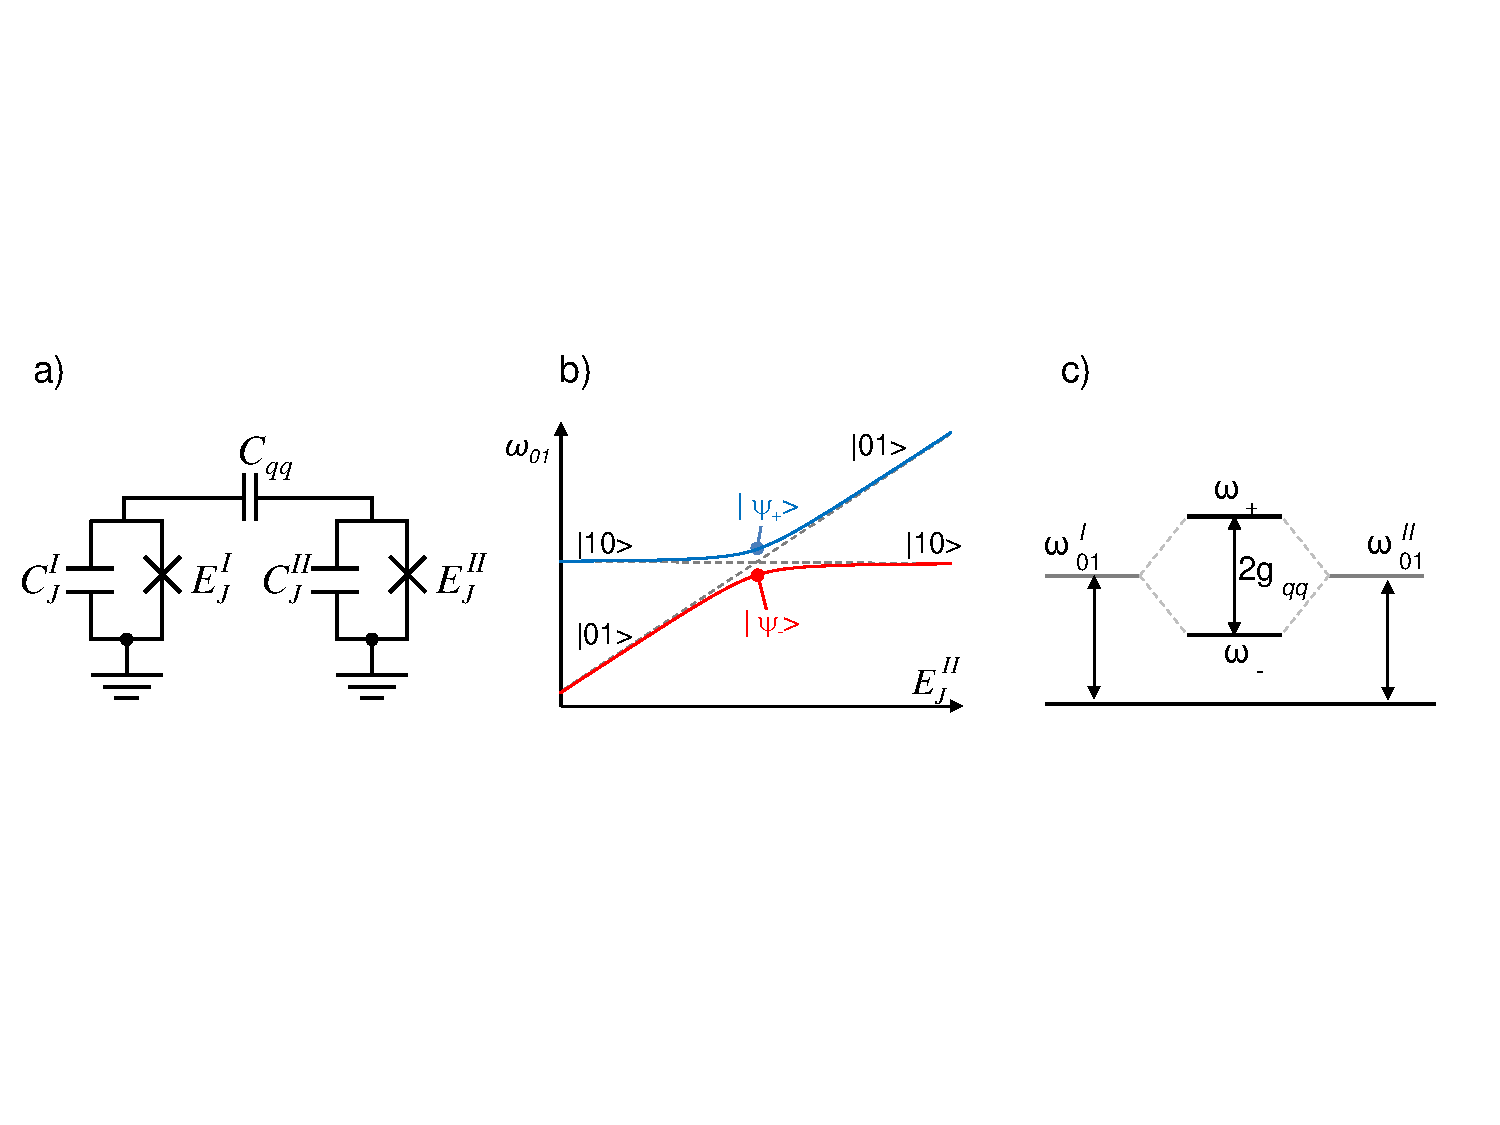
\includegraphics[width=\textwidth]{./material/figures/scalable-architecture/double_transmon_schematic}
	\caption[...]{a)Schematic of the double Transmon qubit, showing two capacitively coupled Transmon qubits. b) Energy level diagram of the double Transmon, showing the eigen-energies of the coupled system as a function of $E_J^{II}$. For $|\omega_{01}^{II}-\omega_{01}^{I}|\gg g_{qq}$, the eigenstates are given as the single-qubit states $\ket{01}$ and $\ket{10}$. For $\omega_{01}^I = \omega_{01}^{II}$, the eigenstates are given as $\ket{\psi_\pm}=(\ket{01}\pm\ket{10})/\sqrt{2}$, with associated eigen-energies $E_\pm = \hbar\omega_\pm = \hbar(\omega_{01}^{I,II}\pm g_{qq})$, as shown in c).}
	\label{fig:qubit_molecule_schematic}
\end{figure}

The Hamiltonian of the double Transmon can be written as
%
\begin{eqnarray}
\hat{H}_{dt}       & = & \hat{H}_q+\hat{H}_{qq} \\
\hat{H}_{q}/\hbar  & = & \omega_{01}^I\hat{\sigma}_z^I+\omega_{01}^{II}\hat{\sigma}_z^{II} \\
\hat{H}_{qq}/\hbar & = & g_{qq}\left(\hat{\sigma}_+^I\hat{\sigma}_-^{II}+\hat{\sigma}_-^I\hat{\sigma}_+^{II}\right) \\
\end{eqnarray}
%
$\hat{H}_{dt}$ (written in the two-state basis $\ket{0}$, $\ket{1}$) consists of the individual Hamiltonians and a coupling Hamiltonian just as the one given by eq. (\ref{eq:cqed_capacitive_coupling}). As before, we can rewrite $\hat{H}_{qq}$ in the eigenbasis $\ket{00}$, $\ket{01}$, $\ket{10}$, $\ket{11}$ of $\hat{H}_q$ as
%
\begin{equation}
\hat{H}_{qq}/\hbar = g_{qq}\left(\ket{10}\bra{01}+\ket{01}\bra{10}\right)
\end{equation}
%
When the qubit frequencies are on resonance such that $\Delta = \omega_{01}^I-\omega_{01}^{II}=0$, the eigenstates of $\hat{H}_{dt}$ are given as $\ket{00}$,$\ket{11}$, $\ket{\psi_+}=1/\sqrt{2}(\ket{01}+\ket{10})$ and $\ket{\psi_-}=1/\sqrt{2}(\ket{01}-\ket{10})$. Far off resonance, where $\Delta \gg g_{qq}$, the eigenstates will correspond to those of $\hat{H}_{qq}$. Now, when coupling both qubits to the cavity with the same coupling constant $g_{01}$, we obtain a coupling Hamiltonian as in eq. (\ref{eq:cqed_bus_coupling}):
%
\begin{equation}
\hat{H}_{qr}/\hbar = g_{01}^I\left(\hat{\sigma}_+^I\hat{a}+\hat{\sigma}_-^I\hat{a}^\dagger\right)+g_{01}^{II}\left(\hat{\sigma}_+^{II}\hat{a}+\hat{\sigma}_-^{II}\hat{a}^\dagger \right). \label{eq:double_transmon_resonator_coupling}
\end{equation}
%
Here, as before, the Hamiltonian of the resonator is given by eq. (\ref{eq:lc_hamiltonian}). As can be seen, the coupling operator between the two qubits and the resonator contains the sums $\hat{\sigma}_+^{I+II}=\hat{\sigma}_+^I+\hat{\sigma}_-^{II}$ and $\hat{\sigma}_-^{I+II}=\hat{\sigma}_-^I+\hat{\sigma}_-^{II}$. Now, writing the coupling Hamiltonian (\ref{eq:double_transmon_resonator_coupling}) in the eigenbasis of $\hat{H}_{qq}$ at $\Delta=0$ yields
%
\begin{equation}
\hat{H}_{qr} = \sqrt{2}g_{01}\left[\left(\ket{11}\bra{\psi_+}+\ket{\psi_+}\bra{00}\right)\hat{a}+\left(\ket{\psi_+}\bra{11}+\ket{00}\bra{\psi_+}\right)\hat{a}^\dagger\right].
\end{equation}
%
As can be seen, the qubit state $\ket{\psi_-}$ does not couple at all to the resonator, whereas the state $\ket{\psi_+}$ couples to it with an enhanced rate $\sqrt{2}g_{01}$ (the states $\ket{01}=(\ket{\psi_+}+\ket{\psi_-})/sqrt{2}$ and $\ket{10}=(\ket{\psi_+}-\ket{\psi_-})/\sqrt{2}$ couple to the at the normal rate $g_{01}$). Thus, if we operate the double Transmon at $\Delta = 0$ and ``park'' the qubit in the state $\ket{\psi_-}$, we can effectively fully switch off the coupling to the resonator. To switch it on and off, we can thus simply peform an adiabatic passage between the states $\ket{\psi_-}$ and $\ket{10}$ \citep{srinivasan_tunable_2011}, using the state $\ket{\psi_-}$ as a logical qubit state. Alternatively, we can induce the transition $\ket{\psi_-}\to\ket{\psi_+}$ by using two single qubit pulses $X^I_\pi Y^{II}_\pi$, which however requires the possibility to drive each of the qubits seperately.

\smallskip

Using this coupling approach elimiates hence the frequency crowding problem and implements a fully controllable, on-demand qubit-qubit coupling scheme. In addition, parking the qubit in the states $\ket{\psi_\pm}$ can reduce dephasing due to first-order flux noise, as explained in chapter \ref{chapter:processor_characterization}. In the following sections we will discuss a possible qubit architecture based on double Transmon, designing as an example a 4-qubit processor.

%When taking into account the second Transmon level $\ket{2}$, the capacitive coupling induces additional coupling elements
%
%\begin{eqnarray}
%\hat{H}_{qq}'/\hbar g_{qq} &  = &  \left(\ket{10}\bra{01}+\ket{01}\bra{10}\right) \\
%& + & \sqrt{2}\left(\ket{11}\bra{02}+\ket{02}\bra{11}\right) \\
%& + & \sqrt{2}\left(\ket{11}\bra{20}+\ket{20}\ket{11}\right) \\
%& + & 2\left(\ket{21}\bra{12}+\ket{12}\bra{21}\right)
%\end{eqnarray}
%
%that we will ignore for now, but which become important when choosing the parameters of the double Transmon.


\section{Designing and Realizing A Four-Qubit Architecture}

\begin{SCfigure}[1.0][ht!]
	\centering
	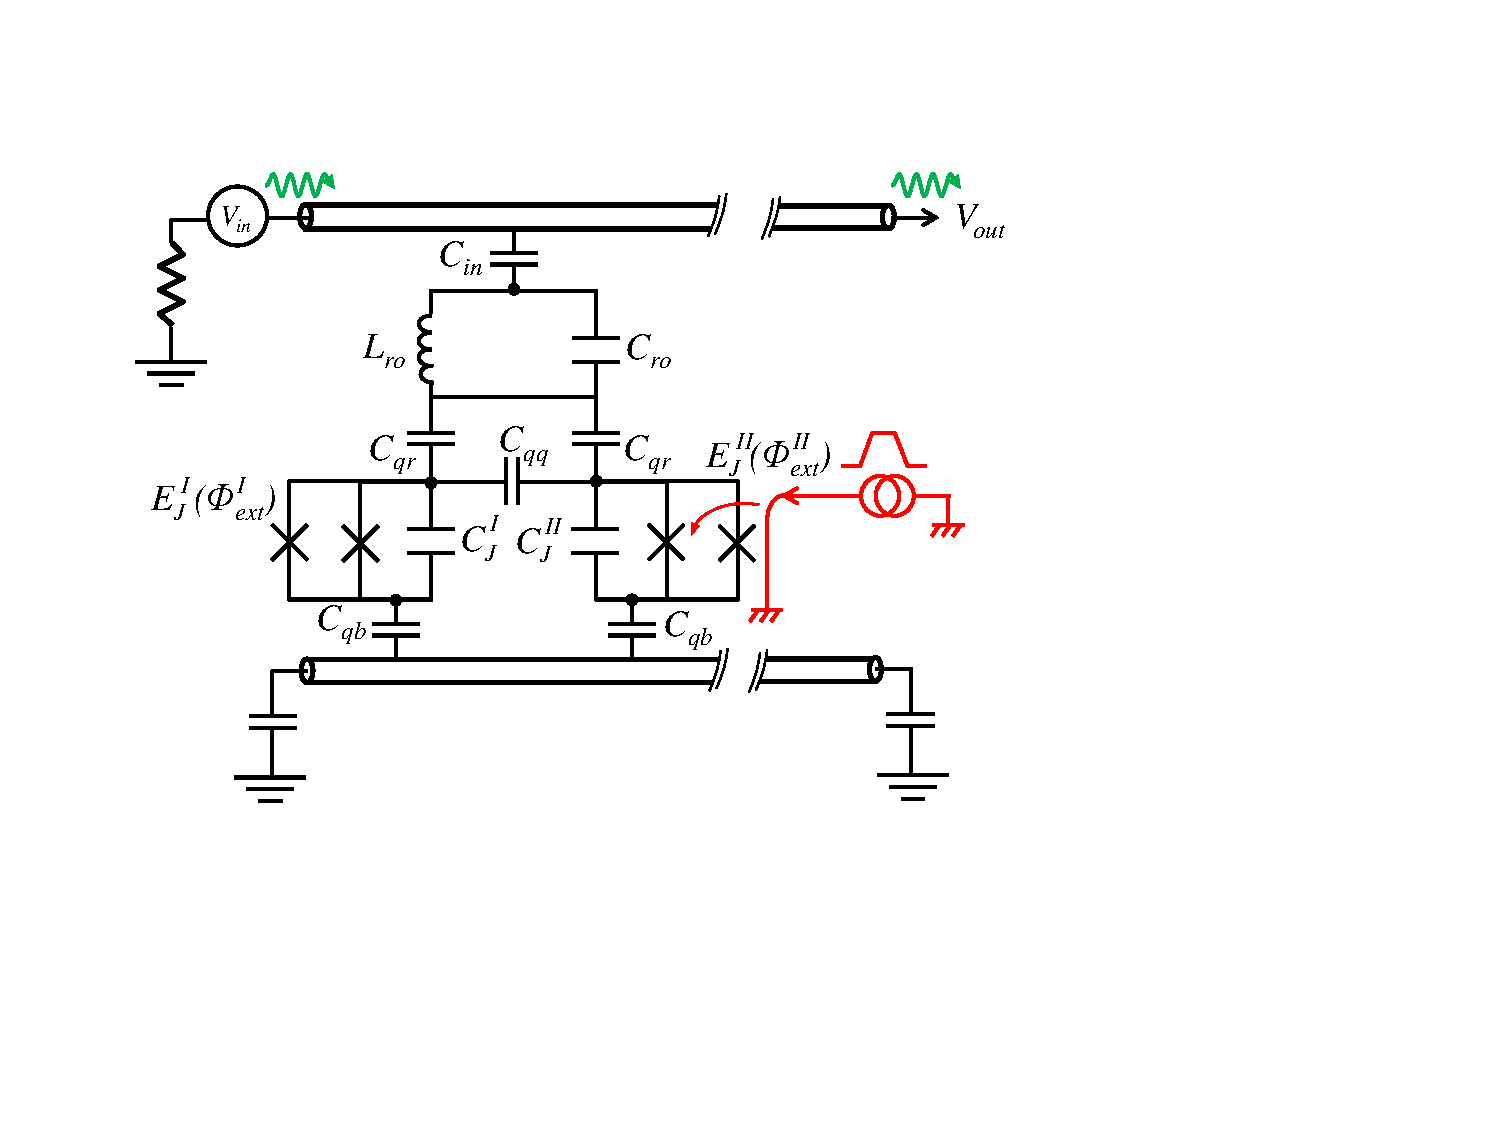
\includegraphics[width=0.6\textwidth]{./material/figures/scalable-architecture/double_transmon_architecture_schematic}
	\caption[]{Schematic of a qubit/readout unit cell of the proposed scalable architecture. Shown is a harmonic resonator capacitively coupled to an input transmission line and to two frequency-tunable Transmon qubits, which are in turn coupled to a coplanar waveguide $\lambda/2$ resonator that acts as a quantum bus to the other qubits. One of the two Transmons is equipped with a fast magnetic flux line.}
	\label{fig:scalable_architecture_schematic}
\end{SCfigure}

Here we describe the design and implementation of a four-qubit architecture using double Transmon qubits, a quantum bus and a invidiual-qubit single shot CJBA readout. The schematic of the proposed architecture is shown in fig. \ref{fig:scalable_architecture_schematic}, showing a double Transmon capacitively coupled to a quantum bus realized as a transmission line resonator and to a CJBA readout resonator, which is in turn capacitively coupled to an input transmission line (please note that for sake of clarity we have omitted the capacitances of the LC resonator and the Transmon qubits to the ground node). As before, each of the Transmons is realized as a split-CPB, thereby making it frequency-tunable through an external flux $\Phi_{ext}^{I,II}$. Since the coupling scheme as discussed in section \ref{section:double_transmon} requires only one of the two Transmons to be fast-frequency tunable, our design includes only one fast flux line per double Transmon. The flux of the other qubit can be tuned to the desired qubit bias point by e.g. using a superconducting coil mounted above it, which can be easily extended to multiple qubits \citep{baur_realizing_2012}.

\smallskip

The capacitive coupling of each of the two qubits to the quantum bus and the readout resonator is identical, which is necessary in order to be able to cancel the qubit-resonator interaction in the state $\ket{\psi_-}$, as discussed in section \ref{section:double_transmon}. The readout resonator itself can be realized either as a lumped-elements resonator or as a distributed transmission line resonator.

\smallskip

To be able to displace the qubit frequencies for readout and multi-qubit coupling without crossing any resonator frequencies, we ``sandwich'' the qubit working frequencies between that of the quantum bus (whose frequency is below all qubit frequencies) and the readout resonators (whose frequencies are above the individual qubit frequencies). For the readout and driving, we use a multiplexed input transmission line. In oder to avoid crosstalk between individual readout resonators when driving them, we displace their frequencies from each other by a small amount, typically 150 MHz. The frequency of the quantum bus is chosen in function of the minimum qubit working frequencies such that the coupling of each qubit to the bus at that frequency is suffciently large to realize a two-qubit gate in a time small compared to the decoherence times of the qubits. Each qubit is then positioned at an optimal working point between the readout resonator and the quantum bus. To perform multi-qubit gates as well as qubit readout, we displace the qubit frequency and bring it either close to the quantum bus (for qubit-qubit coupling) or the readout resonator, as we explain in the following section.

\smallskip

In the following sections, we refer to the individual qubit frequencies of the $i$-th double Transmon as $\omega_{01}^{I,i}$ and $\omega_{01}^{II,i}$ and define $\Delta_i = \omega_{01}^{I,i}-\omega_{01}^{II,i}$. In addition, we denote its two-qubit states $\ket{x}$ it with an exponent $i$, $\ket{x^i}$.

\subsection{Processor Operation}

\begin{figure}[ht!]
	\centering
	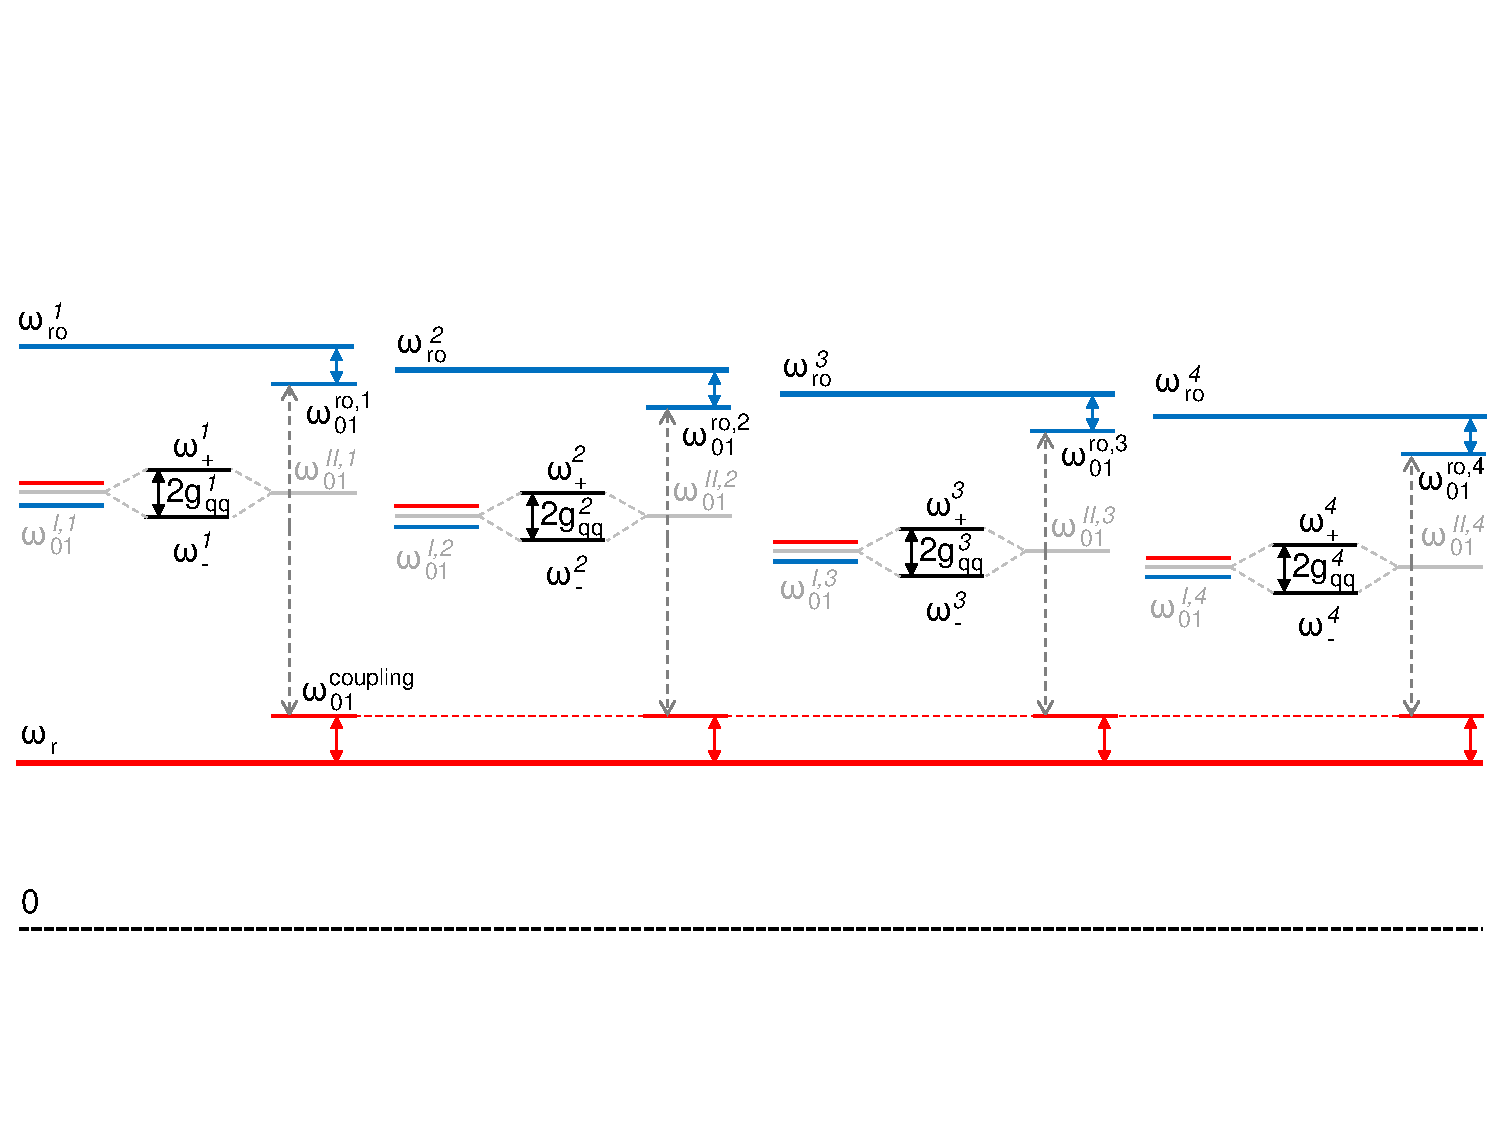
\includegraphics[width=\textwidth]{./material/figures/scalable-architecture/qubit_architecture_energy_levels}
	\caption[]{Operating frequencies of the proposed four-qubit processor, showing the frequencies of the quantum bus, the readout resonators and the four double-Transmon qubits for qubit parking (in black), manipulation (in red) and readout (in blue).}
	\label{fig:scalable_architecture_energy_levels}
\end{figure}

As before, three basic processor operations need to be realized:

\begin{itemize}
\item qubit parking (i.e. no operation)
\item single-qubit gates
\item two-qubit gates
\item qubit readout
\end{itemize}

As for our two-qubit processor, for each of these operations we move the involved qubits to different frequencies, defining hence frequency bands for parking, qubit manipulation and qubit readout, as shown in fig. \ref{fig:}. In the following paragraphs, we explain how we realize each of the operations mentioned above.

\subsubsection{Qubit Parking}

To park a logical qubit $i$, we move it to a frequency $\omega_{01}^{I,i}=\omega_{01}^{II,i}=\omega_{01}^{\mathrm{park}}$ where its computational basis states are given as $\ket{00^i}$, $\ket{\psi_-^i}$, $\ket{\psi_+^i}$, $\ket{11^i}$. Hence, at its parking position the qubit is fully decoupled from the quantum bus and its readout resonator, eliminating thus relaxation through the Purcell effect and decoupling it from all other qubits. 

\subsubsection{Single-Qubit Gates}

To realize single-qubit gates, we perform an adiabatic passage from $\Delta_i = 0$ to $\Delta_i \gg g_{qq}^i$ by chaning $\omega_{01}^{II,i}$, thereby changing the computational basis of the qubit to the states $\ket{00^i}$, $\ket{\tilde{01}^i}\approx \ket{01^i}$, $\ket{\tilde{10}^i}\approx \ket{10^i}$, $\ket{11^i}$. At this point, we can easily drive the $\ket{00^i}\to\ket{10^i}$ transition of the qubit and afterwards perform another adiabatic passage back to the parking position.

\subsubsection{Two-Qubit Gates}

To realize a two-qubit gate between the qubits $i$ and $j$, we adiabatically decrease the frequencies $\omega_{01}^{II,i}$ and $\omega_{01}^{II,j}$ to the point $\omega_{01}^{II,i}=\omega_{01}^{II,j}=\omega_{01}^{\mathrm{coupling}}$. At this frequency there will be a resonant interaction between the logical qubits of the form $\hbar g_{qq}^{ij}(\ket{00^j}\bra{01^i}+\ket{01^j}\bra{00^i})$ with a coupling rate $g_{qq}^{ij}(\omega_{01}^\mathrm{coupling})=g_{01}^i g_{01}^j (\Delta_i^\mathrm{bus}+\Delta_j^\mathrm{bus})/2\Delta_i^{\mathrm{bus}}\Delta_j^\mathrm{bus}$, where $\Delta_i^\mathrm{bus}=|\omega_\mathrm{bus}-\omega_{01}^{II,i}|$. Please note that there will also be a spurious coupling of the same form to the $\ket{00}$ and $\ket{\psi_+}$ states of all other qubits $k$. However, this residual coupling can be made negligibly small by choosing a sufficiently large detuning $\omega_\mathrm{park}-\omega_\mathrm{coupling} \gg g_{qq}^{ij}$, as explained in section \ref{section:qubit_qubit_coupling}. 

\subsubsection{Qubit Readout}

To read out the state of qubit $i$, we perform a gate operation $\ket{\psi_-^i}\to\ket{\psi_+^i}$ by non-adiabatically detuning the qubits to $\Delta_i\gg g_{qq}^i$, letting them evolve for a time $t_\pi=\pi/(|\omega_{01}^{I,i}-\omega_{01}^{II,i}|)$, non-adiabatically tuning them back to $\Delta_i = 0$ and then performing an adiabatic passage to the state $\ket{01}$ by increasing $\omega_{01}^{II,i}$ to $\omega_{01}^\mathrm{ro,i}$, the optimal readout frequency for qubit $i$.

\subsection{Design Parameters}

As before, we need to choose the maximum transition frequency $f_{01}^{max}$ and anharmonicity as well as the junction asymmetry for the double Transmon. The choice of these parameters has been discussed in detail in chapter \ref{chapter:design}. In addition, we need to choose the qubit-qubit coupling $g_{qq}$ and the qubit-resonator couplings $g_{qr}$, for which we take into account the following criteria:

\begin{itemize}
\item The coupling should be sufficiently large to be able to drive the $\ket{00}\to\ket{\psi_-}$ transition of the qubit without exciting the $\ket{00}\to \ket{\psi_+}$ transition as well. If, as before, we choose at a maximum Rabi frequency of 100 MHz, we require $g_{qq}/2\pi\ge 100\;\mathrm{MHz}$.
\item The coupling should be large enough to be able to perform an adiabatic transition $\ket{\psi_-}\to\ket{01}$ in a time which is small compared to the relaxation and dephasing times of the qubit. The probability of a diabatic transition when ramping the qubit-qubit detuning $\Delta=\omega_{01}^I-\omega_{01}^{II}$ with the rate $\dot{\Delta}=\partial \Delta/\partial t$ is given by the Landauer-Zener formula $P_d(\dot{\Delta})=\exp{-2\pi g_{qq}^2/\dot{\Delta}}$. In order to perform an adiabatic transition from $\Delta=0$ to $\Delta = 10g_{qq}$ in $10\;\mathrm{ns}$ (which is sufficiently short compared to relaxation and dephasing times) with a diabatic probability $P_d<1\%$, we need $g_{qq}/2\pi\ge 116\;\mathrm{MHz}$. 
\end{itemize}

\subsection{Implementation}

\begin{figure}[ht!]
	\centering
	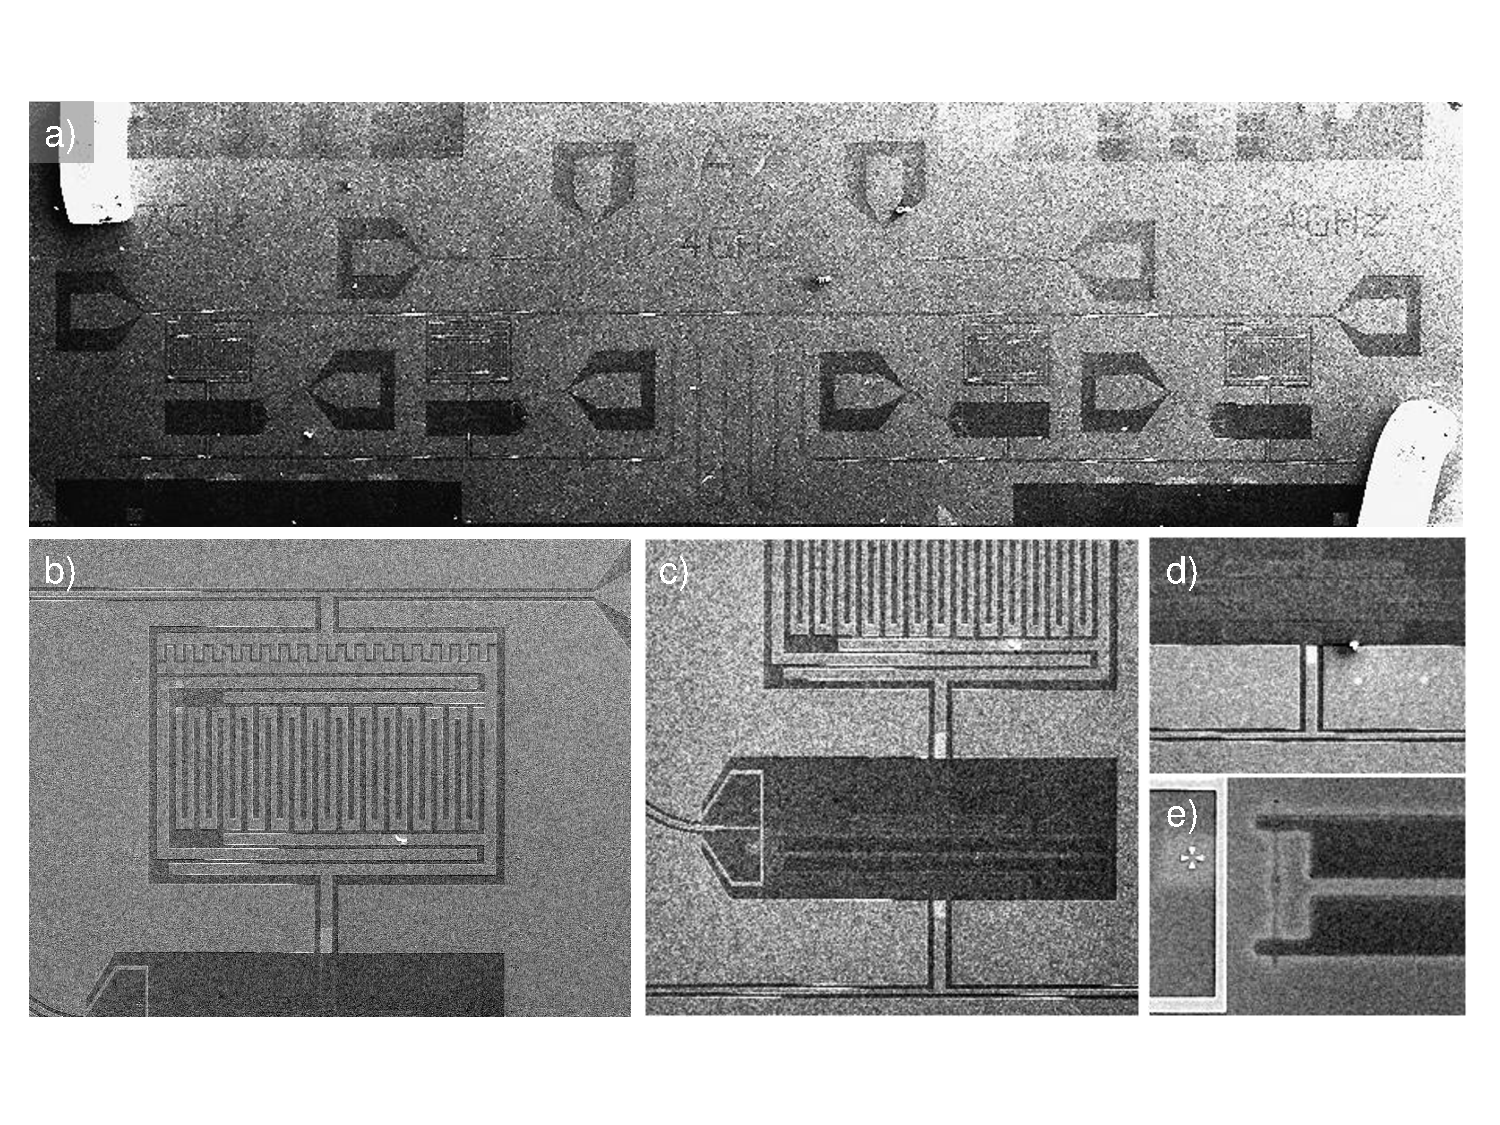
\includegraphics[width=\textwidth]{./material/figures/scalable-architecture/scalable_architecture_photos}
	\caption[]{Photos of the realized four-qubit chip. a) A stitched together image of the whole chip, showing the input transmission line, the readout resonators, qubit cells, fast flux lines and quantum bus. b) A detailed view of a single readout resonator, showing the CJBA realized in lumped elements and capacitively coupled to the input transmission line (above) as well as the qubit cell (below). c)A detailed view of a single Transmon qubit, which is capacitively coupled to its readout resonator and the quantum bus. The Transmon SQUID is inductively coupled to a fast flux line. d) The bus coupling capacitance of a single qubit. e) A detailed view of the qubit capacitance and SQUID as well as the adjacent fast flux line.}
	\label{fig:scalable_architecture_photos}
\end{figure}

\section{Scalability \& Comparison to Current Development}

\subsection{3D Circuit Quantum Electrodynamics}

\subsection{Hybrid Quantum Systems}
